\documentclass{article}

\PassOptionsToPackage{square,numbers}{natbib}

\usepackage[final]{neurips_2024}


% to compile a preprint version, e.g., for submission to arXiv, add add the
% [preprint] option:
%     \usepackage[preprint]{neurips_2024}


% to compile a camera-ready version, add the [final] option, e.g.:
%     \usepackage[final]{neurips_2024}


% to avoid loading the natbib package, add option nonatbib:
%    \usepackage[nonatbib]{neurips_2024}


\usepackage[utf8]{inputenc} % allow utf-8 input
\usepackage[T1]{fontenc}    % use 8-bit T1 fonts
\usepackage{hyperref}       % hyperlinks
\usepackage{url}            % simple URL typesetting
\usepackage{booktabs}       % professional-quality tables
\usepackage{amsfonts}       % blackboard math symbols
\usepackage{nicefrac}       % compact symbols for 1/2, etc.
\usepackage{microtype}      % microtypography
\usepackage{xcolor}         % colors

\usepackage{csquotes}
\usepackage{graphicx}
\usepackage{amsmath}
\usepackage{multirow}


\title{Sentiment Analysis on Movie Reviews [Mini]}


\author{
  Maël Dieudonné\\
  ENSAE\\
  \texttt{mael.dieudonne@ensae.fr} \\
}


\begin{document}

\maketitle

\begin{abstract}
Sentiment analysis aims to capture the subjectivity expressed in written texts. It is most commonly performed at the document level using a binary approach---classifying the overall emotional tone as either positive or negative. This method is frequently applied to movie reviews, which tend to be longer and more readily available than other subjective texts, such as product reviews.

The dataset in question, published in 2011, consists of 50,000 IMDb movie reviews labeled as either positive or negative based on their associated rating (respectively 7 or higher and 4 or lower; reviews associated with ratings of 5 and 6 were deliberately excluded).

Current SOTA models on this dataset are fine-tuned encoders, but their performance seems to have reached a plateau. Replicating these models would require excessive computational resources. Instead, I have chosen to investigate an alternative explanation: that this plateauing is due to limitations within the dataset itself.

I compared the performances of 4 models: 3 based on RoBERTa (the base model, my own fine-tuned version trained on the IMDb dataset, and a SOTA model fine-tuned specifically for sentiment analysis) and GPT-3.5 Turbo. All models exhibit a significant drop in accuracy for reviews with ratings of 4 and 7. Combined with a cursory examination of the dataset, this suggests that ratings may not be an optimal proxy for the sentiment expressed in movie reviews. If so, this could introduce noise into the true labels, making perfect prediction inherently unattainable.
\end{abstract}


\section{Introduction}

Sentiment analysis seeks to understand the subjectivity expressed in written documents. Opinion and views are often used interchangeably with sentiment in the literature, in contrast to factual statements \citep{munezero_are_2014}.

Sentiment analysis has become an active research area with the advent of Web 2.0, offering people numerous opportunities to express themselves in a publicly traceable manner \citep{stine_sentiment_2019}. Various stakeholders have a vested interest in their opinions:
\begin{itemize}
    \item \textbf{Marketing departments}, seeking to understand brand perception and consumer opinions about products, both in absolute terms and relative to competitors.
    \item \textbf{Customer service teams}, identifying key factors contributing to customer satisfaction or dissatisfaction.
    \item \textbf{Traders and financial analysts}, using public sentiment as an early indicator of economic trends and the financial health of companies.
    \item \textbf{Political actors}, monitoring public perception of policies and personal image.
    \item \textbf{Public health officials}, assessing attitudes toward medical interventions such as vaccines.
    \item Etc.
\end{itemize}

The primary goal of sentiment analysis is to gain direct access to people's opinions without relying on intermediaries such as journalists or resellers, at the massive scale typical of the Internet \citep{ravi_survey_2015,hemmatian_survey_2019}.

Sentiment analysis can be performed at three distinct levels. At the \textbf{document level}, the goal is to determine the overall sentiment of an entire document, which can be very short (e.g., product reviews). Analysis conducted at the \textbf{sentence level} account for potentially conflicting sentiments within the same documents. First, it distinguishes between objective (fact-based) and subjective (opinion-based) sentences. For example, a movie review may contain both plot summaries (objective) and judgments on acting performance (subjective). Then, subjective sentences are classified based on their sentiment. At the \textbf{feature} or \textbf{aspect level}, the aim is to link sentiments with their object, and sometimes the person expressing them (who feels what about the plot, for instance).

The most common output of sentiment analysis is a binary or ternary classification of the emotional tone, also known as polarity or valence: positive, negative or neutral. This classification applies to entire documents, individual subjective sentences, or specific features, depending on the level of analysis. Sentiment classification beyond polarity, aiming at identifying specific emotions like fear, anger, or happiness, is less common. This approach may have fewer applications outside of literary analysis.

Sentiment analysis faces several important challenges \citep{kumar_comprehensive_2023}:
\begin{itemize}
    \item \textbf{Domain dependance}, when words carry different meanings in different contexts (e.g., tears may indicate laughter or sadness).
    \item \textbf{Polarity shift}, when words or punctuation marks change the valence of a sentiment (e.g., not, but, only).
    \item \textbf{Sarcasm}, when the expressed sentiments oppose the actual sentiments.
    \item \textbf{Order dependance}, when the valence of a word changes with its position in the sentence (e.g., with comparisons).
    \item \textbf{Unconventional expressions} like idioms, slang, emojis, or multiple punctuations marks.
Implicit sentiment, when sentiments are expressed without explicit sentiment words (e.g., \enquote{I know real Indian food and this wasn’t it}).
\end{itemize}


\section{State of the art}

Three main approaches have been applied to sentiment analysis, making use of lexicon-based models, classifiers, and transformers \citep{hartmann_more_2023}.

\subsection{Lexicon-based}

This approach relies on a dictionary assigning positive or negative labels to words, to classify documents based on the most frequent label. A well-known example is VADER, which was developed to analyze the sentiments of reviews published on social media \citep{hutto_vader_2014}. It relies on sentiment lexicon of 7,520 words including slang, emoticons, and acronyms, where each word is associated with a score on a valence scale (e.g., -2.2 for \enquote{:(}, 0.9 for \enquote{okay} or 3.1 for \enquote{good}). This lexicon was obtained by submitting a list of 9,000 words to human raters recruited on the Amazon Mechanical Turk. Each word was rated by 10 different persons on a 9-point Likert scale, and kept in the lexicon if its average rating was non-null. VADER also applies rules that adjust sentiment scores based on punctuation, capitalization, and specific words (e.g., \enquote{but} shifts sentiment, while \enquote{!!} amplifies intensity). Finally, VADER calculates the proportion of text conveying positive, negative, or neutral sentiment.

This approach has several limits. Lexicons are complex to build, as they require a lot of human input, so they tend to remain small and not updated very often. They also lack flexibility, being unable to handle words they do not include. This can be especially problematic when processing content drawn from the Internet, which may include words written incorrectly or with evolving meaning. Since the analysis occurs at the word level, it lacks contextual understanding. As a result, the performance of lexicon-based sentiment analysis is rather low.

\subsection{Classifiers}

A second approach consists of using standard machine learning algorithms. Almost any classification algorithm can be applied; the challenge lies in preprocessing the text to make it suitable for the classifier, typically through a bag-of-words representation. This method produces a high-dimensional but sparse feature space, making regularization techniques particularly useful. These techniques reduce the vocabulary—similar to a lexicon—but do so based on a word’s effectiveness in sentiment prediction rather than a predefined list. An example is available here with support vector machines, random forest and neural networks \citep{wang_is_2024}.

The use of classifiers can be seen as a generalization of lexicon-based approaches. Unlike lexicon-based methods, classifiers do not require a predefined dictionary specifying which words to consider and how to interpret them. Instead, models autonomously select the words they rely on for classification, along with their associated sentiment (i.e., emotional tone). They enable more complex mappings between the input (i.e., document) and the output (i.e., predicted sentiment) beyond simple relative word frequencies. Classifiers can also incorporate external features, such as a reviewer’s personal characteristics, to refine predictions.

However, classifiers have limitations. They require labeled datasets to train the models, though these datasets are generally easier to construct than sentiment dictionaries. Despite their advantages, classifiers may still struggle with understanding connotations and context, as they analyze words in isolation. While they perform well on short documents, they often have difficulty handling longer texts that express conflicting viewpoints.

\subsection{Transformers}

The third approach uses transformer models, which apply attention mechanisms to word embeddings—low-dimensional, dense representations of text. There are two main types of models sharing the same basic architecture:
\begin{itemize}
    \item \textbf{Encoder/decoder} (a.k.a. unidirectional or autoregressive transformers): these models consider only past and present tokens, with the aim of predicting future tokens (which are removed from through causal masking). They are easily trained by comparing predicted and actual tokens. The reference architecture for encoders/decoders is GPT \citep{radford_improving_2018,radford_language_2019}.
    \item \textbf{Encoder-only} (a.k.a. bidirectional transformers): these models consider all tokens in the context window, with the aim of understanding text. They are trained by masking a fraction of input tokens (usually 15\%) before feeding them to the model, then predicting the masked tokens. Additional training strategies include predicting the order of two sequences in the training corpus or generating permutations of tokens within sentences. Lacking decoders, these models output embeddings instead of tokens. These embeddings can be analyzed directly, e.g., through cosine similarity to identify semantically similar tokens, which is essentially the principle of \textbf{zero-shot classification}. Alternatively, a custom output head can be added and fine-tuned for a specific task. The reference architecture of encoders is BERT \citep{devlin_bert_2019}.
\end{itemize}

Large language models offer powerful tools for sentiment analysis, with a unique ability to capture context and disentangle sentiment from other features. They excel in complex tasks, particularly aspect-based sentiment analysis. However, they have several limitations. They are resource-intensive, especially during pre-training. As a result, the most common approach is to use pre-trained encoders models, either directly or for fine-tuning. A less frequent approach is to run GPT models locally or access them via APIs. Another challenge with transformers is their opacity; what makes them so effective remains difficult to assess. Lastly, they may not outperform traditional classifiers on short documents \citep{ghatora_sentiment_2024}.


\section{Data}

Movie reviews have become a popular benchmark for sentiment analysis due to their availability and size: they tend to be longer and more accessible online compared to typical product reviews or social media posts. The current dataset was constructed and publicized by Maas et al. \citep{maas_learning_2011}. It contains 50,000 reviews from the IMDb website, along with the corresponding rating proposed by theirs authors on a 1-10 scale. Reviews are labeled as negative when associated with ratings below 5, as positive when associated with ratings above 6. Neutral ratings (5 and 6) were eliminated to focus on polarized reviews. To minimize bias, no more than 30 reviews per movie were included, and an equal number of positive and negative reviews were selected, ensuring that random guessing would yield 50\% accuracy. The dataset is split into training and test samples of equal size (25,000 reviews each) 
\footnote{The dataset also includes an additional 50,000 unlabeled reviews without ratings. These can be used for unsupervised learning but not to measure performance.}
.

\textbf{The task, therefore, is to perform binary classification between positive and negative sentiments at the document level.}

\subsection{Benchmarks}

Performances are assessed regarding accuracy, which is the most relevant metrics for a binary classification problem where each class is of equal importance and the dataset is balanced. This is different from, e.g., diagnosing a serious but rare disease, where false positives are preferable to false negatives, and recall would be the performance metric of choice.

Several models were benchmarked on the IMDb dataset, reaching the following error rates on the test sample \citep{stine_sentiment_2019}:
\begin{itemize}
    \item 26.4\% for a \textbf{lexicon-based model},
	\item 12.3\% for a \textbf{Lasso logistic regression},
	\item 5.91\% for an \textbf{adversarial neural network}.
\end{itemize}

The current best model (according to the \href{https://paperswithcode.com/sota/sentiment-analysis-on-imdb}{Papers with Code leaderboard}) is a \textbf{fine-tuned BERT} model named LlamBERT (Csanády et al., 2024) with an error rate of 3.32\%. It is followed closely by an \textbf{auto-regressive transformer} named XLNet (Yang et al., 2019) with an error rate of 3.79\%.

Transformers are significantly outperforming lexicon-based models and traditional classification algorithms. This is not surprising, as they leverage much more information, being trained on corpora orders of magnitude larger than the IMDb dataset. However, they seem to have reached a plateau, with only marginal improvements over the last 6 years. Additionally, they are difficult to replicate due to heavy hardware requirements. It seems clearly out of my reach to improve upon these models.

\section{Experiment}

\subsection{Hypotheses}

Instead, I have set out to investigate the possibility that performance is plateauing due to limitations of the dataset, with two hypotheses in mind.

(1) The way reviews are labeled means that the prediction task is not based on the sentiment conveyed by reviews, but on the associated ratings (below 5 or above 6). However, these ratings may not always be a reliable proxy for the overall sentiment of reviews, especially when they are not strongly polarized. Below are a few examples of reviews labeled as positive, despite their tone being quite ambiguous:

\begin{displayquote}
Definitely a movie that could've been seen on DVD. (rating 7)

Moviegoers wanting an inside look at what it's like to embark on a daring rescue mission in the middle of the ocean might want to give The Guardian a chance. I saw it for free, but had I paid I would've felt I had gotten my money's worth. (rating 8)

In the end, "The Dresser" will bore many people silly, but it will truly be a delight to those who love British cinema. (rating 8)

The theme is controversial and the depiction of the hypocritical and sexually starved india is excellent.Nothing more to this film.There is a lack of good dialogues(why was the movie in english??). There was lack of continuity and lack of passion/emotion in the acting. (rating8)
\end{displayquote}
The working hypothesis here is that the error rate is higher for models closer to neutral, especially with a rating of 7.

(2) The document-level approach is not ideal, as many reviews express conflicting opinions about different aspects of a movie, making it difficult to assign a single, reliable sentiment.

\begin{displayquote}
Some things and some actions are very true, but some other stuff is just way off the mark. (…) Delhi is complicated. India is complicated. The director tries to simplify both. And fails pretty miserably at that. (…) But the chemistry between the leads is palpable. (rating 8)

The plot is rather thin, yet it does have a moral. It's about the perils of quick fame and fast money, and how any happiness with only these factors will ultimately be doomed. This will cheer you up, lift you up to your feet and make you laugh. (…) Another major problem is that too many songs are just not that great. (…) The grandmother sub-plot borders on being ridiculous. (rating 8)
\end{displayquote}
The working hypothesis here is the lengthier the reviews, the more likely they are to express contrasted opinions, and the harder they become to classify.

\subsection{Models}

My goal was to compare several models to assess their behavior in relation to ratings and review lengths, while striving to get as close as possible to the SOTA performance. I chose RoBERTa Large \citep{liu_roberta_2019} as my base model , since the SOTA model is built upon it and it also performs really well on its own (outperforming XLNet, which serves as the basis for the second SOTA model) 
\footnote{It could have been interesting to use ModernBERT \citep{warner_smarter_2024} instead, which is more recent, but I discovered its existence too late.}
.

RoBERTa's architecture is largely similar to the original BERT model, with only minor tweaks to some hyperparameters. It has a vocabulary size of 50,265, a hidden size of 768 for RoBERTa base and 1024 for RoBERTa large, 12 attention heads with 12 layers each and an intermediate size of 3072. The context length is 512 tokens. The sole difference between BERT and RoBERTa architectures regards tokenization. RoBERTa uses Byte-Pair Encoding, which operates at the subword level with an agglomerative approach, merging the most frequent pairs iteratively until the desired vocabulary size is reached. Additionally, RoBERTa omits \texttt{token\_type\_ids}, which are used in BERT to distinguish between prompts and answers.

Where BERT and RoBERTa truly differ is in their training procedures. RoBERTa eliminates the next sentence prediction objective and employs dynamic masking, meaning that input tokens are masked differently every 4 epochs rather than being fixed during preprocessing. Additionally, RoBERTa's training algorithm uses larger mini-batches and significantly fewer training steps (30,000 compared to 1 million for BERT). Its training corpus is also substantially larger, at approximately 160 GB. While I could not confirm whether it includes the IMDb dataset, it does use OpenWebText, which is built from content extracted from URLs shared on Reddit with at least 3 upvotes.

I use zero-shot classification with the base RoBERTa model through a simple HuggingFace pipeline as a baseline for performance, comparing it with the following models.

\subsubsection{Fine-tuned RoBERTa on the IMDb dataset}

I used a custom classification head with… 
\begin{itemize}
    \item A dense layer mapping RoBERTa output to a hidden space of similar size (making for \( 1024*1024+1024=1,049,600 \) trainable parameters)
	\item A drop-out layer with a rate of 0.1 to prevent overfitting
	\item An activation layer with GELU (same as RoBERTa) to introduce non-linearities
	\item A normalization layer (making for \( 1024*2=2,048 \) trainable parameters)
	\item A dense layer reducing the hidden space dimension by a factor 2 (making for \(1024*512+512=524,800\) trainable parameters)
	\item Another dropout layer with the same rate
	\item A final dense layer projecting the hidden space in 2 dimension, corresponding to binary outcomes (making for \(512*2+2=1,026\) trainable parameters)
\end{itemize}
This classification head has 1,577,474 trainable parameters in total, compared with 354,315,266 parameters in RoBERTa-large. It is applied to the \texttt{[CLS]} token, which marks the beginning of input sequences and serves as an embedding for their entirety
\footnote{I have tried applying it to the whole input sequence, pooling tokens through their mean or max, on a subset of reviews: the performance were worse.}
.

Parameters from the base model were frozen to preserve the knowledge acquired during pretraining and avoid excessive computation times. The fine-tuning was conducted with the following settings:
\begin{itemize}
    \item 12 epochs, with performance evaluation on the entire test sample after each epoch to detect overfitting as soon as possible.
	\item An \texttt{AdamW} optimizer with a learning rate of 1e-4, \texttt{weight\_decay} of 0.03, and \texttt{epsilon} set to 1e-6.
    \item A cosine learning rate scheduler with 10\% warmup steps.
\end{itemize}

\subsubsection{SOTA fine-tuned RoBERTa for sentiment analysis}

To assess the effectiveness of my fine-tuning, I compared it not only to the baseline performance but also to the current SOTA fine-tuned RoBERTa for sentiment analysis, which is SiEBERT \citep{hartmann_more_2023}. Its architecture is not specified, as the authors do not describe it and have not released their code. It is unclear whether SiEBERT uses a custom classification head or the default untrained head provided by RoBERTa, which consists of two dense layers (the first mapping to a hidden space of the same size as the RoBERTa output, the second to a binary space). The training corpus is also unspecified; the authors only mention using all publicly available two-class sentiment datasets they could identify, excluding their training subset.

SiEBERT is available in a HuggingFace pipeline, which I used.

\subsubsection{GPT 3.5 turbo}

I decided to add a comparison with ChatGPT, which has shown promising results for sentiment analysis but has never been applied to the IMDb dataset \citep{wang_is_2024}. I drafted a first prompt based on the principle of few-shot prompting, which consists in including a few examples before the document to classify. This has been observed to improve the performance of sentiment analysis significantly—an effect known as in-context learning \citep{brown_language_2020}. I then submitted this prompt to ChatGPT, asking for improvements, and received the suggestion of adding detailed instructions. Prompts were constructed as follows for each review of the test sample:

\begin{displayquote}
Here is an example of a positive movie review, associated with a rating of 10:

*[ \textit{<random review with a positive sentiment from the training set>} ]*

Here is an example of a negative movie review, associated with a rating of 2:

*[ \textit{<random review with a negative sentiment from the training set>} ]*

Now, consider the following review. Based on its content, is the sentiment of the review positive or negative? Answer with a single word.

*[ \textit{<review to classify from the test sample>} ]*

Instructions:

- **Positive** reviews typically highlight enjoyment, satisfaction, or praise for aspects of the film (e.g., acting, storyline, direction).

- **Negative** reviews tend to criticize the film for its shortcomings or failures (e.g., poor pacing, bad acting, or unsatisfying plot).

- Focus on the general tone of the review as a whole, not isolated statements or minor contradictions.
\end{displayquote}

I queried ChatGPT through the OpenAI API. I chose GPT 3.5 Turbo as the best compromise between cost and performance. At \$0.5 per million input tokens and \$1.5 per million output tokens, with 25,582,485 input tokens from building the prompt and 25,000 expected output tokens, the estimated cost was \$12.83.

An inherent challenge with this approach is data leakage. There is a high likelihood that the IMDb test sample was included in GPT-3.5 Turbo's training corpus, which could lead to overestimated performance, as it may not be working with truly unseen data. The solution would have been to build a new dataset by scrapping reviews published after the cutoff date of GPT 3.5 Turbo, which is September 2021, but this would have added significant complexity to the project. Instead, I assumed that the IMDb dataset is small enough to be diluted in the larger training corpus of GPT-3.5 Turbo, making significant memorization unlikely.

\subsection{Data preprocessing}

Text was cleaned consistently across all models to ensure comparability of their results:
\begin{itemize}
    \item Removing HTML markups, primarily line breaks (replacing \texttt{<br>} with \texttt{\textbackslash n} to preserve the paragraph structure).
	\item Removing a few emojis that are not linked to sentiment (® and ©).
    \item Replacing hexadecimal characters by their ASCII equivalent.
\end{itemize}

\section{Results}

\subsection{Data}

Two characteristics of the dataset are not mentioned in the documentation but nonetheless crucial.
\begin{enumerate}
    \item A cursory examination suggests that movies are different in each dataset, even if they share the same id. This is excellent for preventing data leakage between train and test samples.
	\item All reviews goes in pair, with each movie having exactly one positive and one negative review. This forbids the models from learning non-sentiment-related features (e.g., related to the plot of a movie having overwhelmingly positive reviews in the dataset).
\end{enumerate}

The reviews are highly polarized, with nearly half of the dataset consisting of ratings of 1 or 10. The distribution of ratings is almost identical in both the train and test samples. Most reviews are relatively short, but there is a long tail in the distribution of review lengths. Some reviews are exceedingly long, with a maximum of 2,459 words (for an average of 231 words in the train sample, 223 in the test sample). Review length and ratings are almost uncorrelated, with a Pearson correlation coefficient of 0.0148. This indicates that my two hypotheses can be tested independently.

\subsection{Candidate Labels for Zero-Shot classification with RoBERTa}

The initial run with \enquote{positive} and \enquote{negative} as candidate labels yielded relatively low accuracy. To improve performance, I experimented with more informative candidate labels. The best results were achieved using \enquote{good movie} and \enquote{bad movie} as labels, which resulted in an improvement of nearly 7 percentage points in accuracy compared to the \enquote{positive} and \enquote{negative} labels (see Table~\ref{tab:labels_zero_shot}).

\begin{table}
  \caption{Performance of various candidate labels for zero-shot classification with RoBERTa}
  \label{tab:labels_zero_shot}
  \centering
  \begin{tabular}{lc}
    \toprule
    \textbf{Candidate Labels} & \textbf{Accuracy} \\
    \midrule
    positive sentiment / negative sentiment & 0.83056 \\
    positive / negative & 0.85908 \\
    favorable opinion / unfavorable opinion & 0.87596 \\
    positive review / negative review & 0.89136 \\
    excellent / terrible & 0.91140 \\
    good movie / bad movie & 0.91708 \\
    \bottomrule
  \end{tabular}
\end{table}

\subsection{Truncation}

RoBERTa models have a context length of 512 tokens, but many reviews are longer than that. The easiest solution is to truncate them, even though that means loosing part of the information on their overall sentiment. This truncation can be made from the right, keeping the end beginning of sequences, or from the left, keeping the end of input sequences. This could have significant consequences depending on the order in which information is presented in the reviews (e.g., if users always start with positive aspects, and always end with negative aspects).

\begin{table}
  \caption{Effects of truncation side on performance}
  \label{tab:truncation}
  \centering
  \begin{tabular}{lcc}
    \toprule
    \textbf{Model} & \textbf{Left side} & \textbf{Right size} \\
    \midrule
    RoBERTa & 0.9171 & 0.9160 \\
    SiEBERT & 0.9573 & 0.9559 \\
    \bottomrule
  \end{tabular}
\end{table}

Left-side truncation yielded marginally better results (using \enquote{good movie} and \enquote{bad movie} as candidate labels for RoBERTa, see Table~\ref{tab:truncation}). This could be explained by the tendency of some users to summarize their sentiment at the end of their reviews: such summaries would be lost with right-truncation, erasing important information. Although the overall effect is really tenuous, I retained left-side truncation for the fine-tuned RoBERTa model. It was also used in the previous comparison between candidate labels.

\subsection{Fine-tuning}

It was done on a MacBook Pro with an M2 Max equipped with 38 GPU cores and 64 GB of shared memory, using the MPS backend of PyTorch. Its performance significantly outpaced the 16 GB Tesla T4 available in the Datalab. Fine-tuning took approximately 1 hour per epoch (inference time was obviously much lower but still notable: zero-shot classification with RoBERTa took about 30 minutes, sentiment analysis with SiEBERT about 20 minutes). 

During the first training run, train and test losses improved simultaneously until the final (12\textsuperscript{th}) epoch. I then extended the training to 20 epochs, as the model was still learning. Although test loss continued to decrease, the performance gains were clearly plateauing, suggesting that further training would likely yield negligible improvements (see Figure~\ref{fig:roberta-learning-1} 
\footnote{The behavior of the batch test loss can be attributed to the fact that test batches were not shuffled, unlike the training batches. It is quite obvious that some batches are more difficult to classify than others. However, since this only affects the validation stage, it does not interfere with the training process. What is interesting, nonetheless, is that the difference between test batches tends to grow with each epoch, as if the model was improving for certain batches while plateauing on others.}
). As a result, I decided to stop training at that point.

\begin{figure}
  \centering
  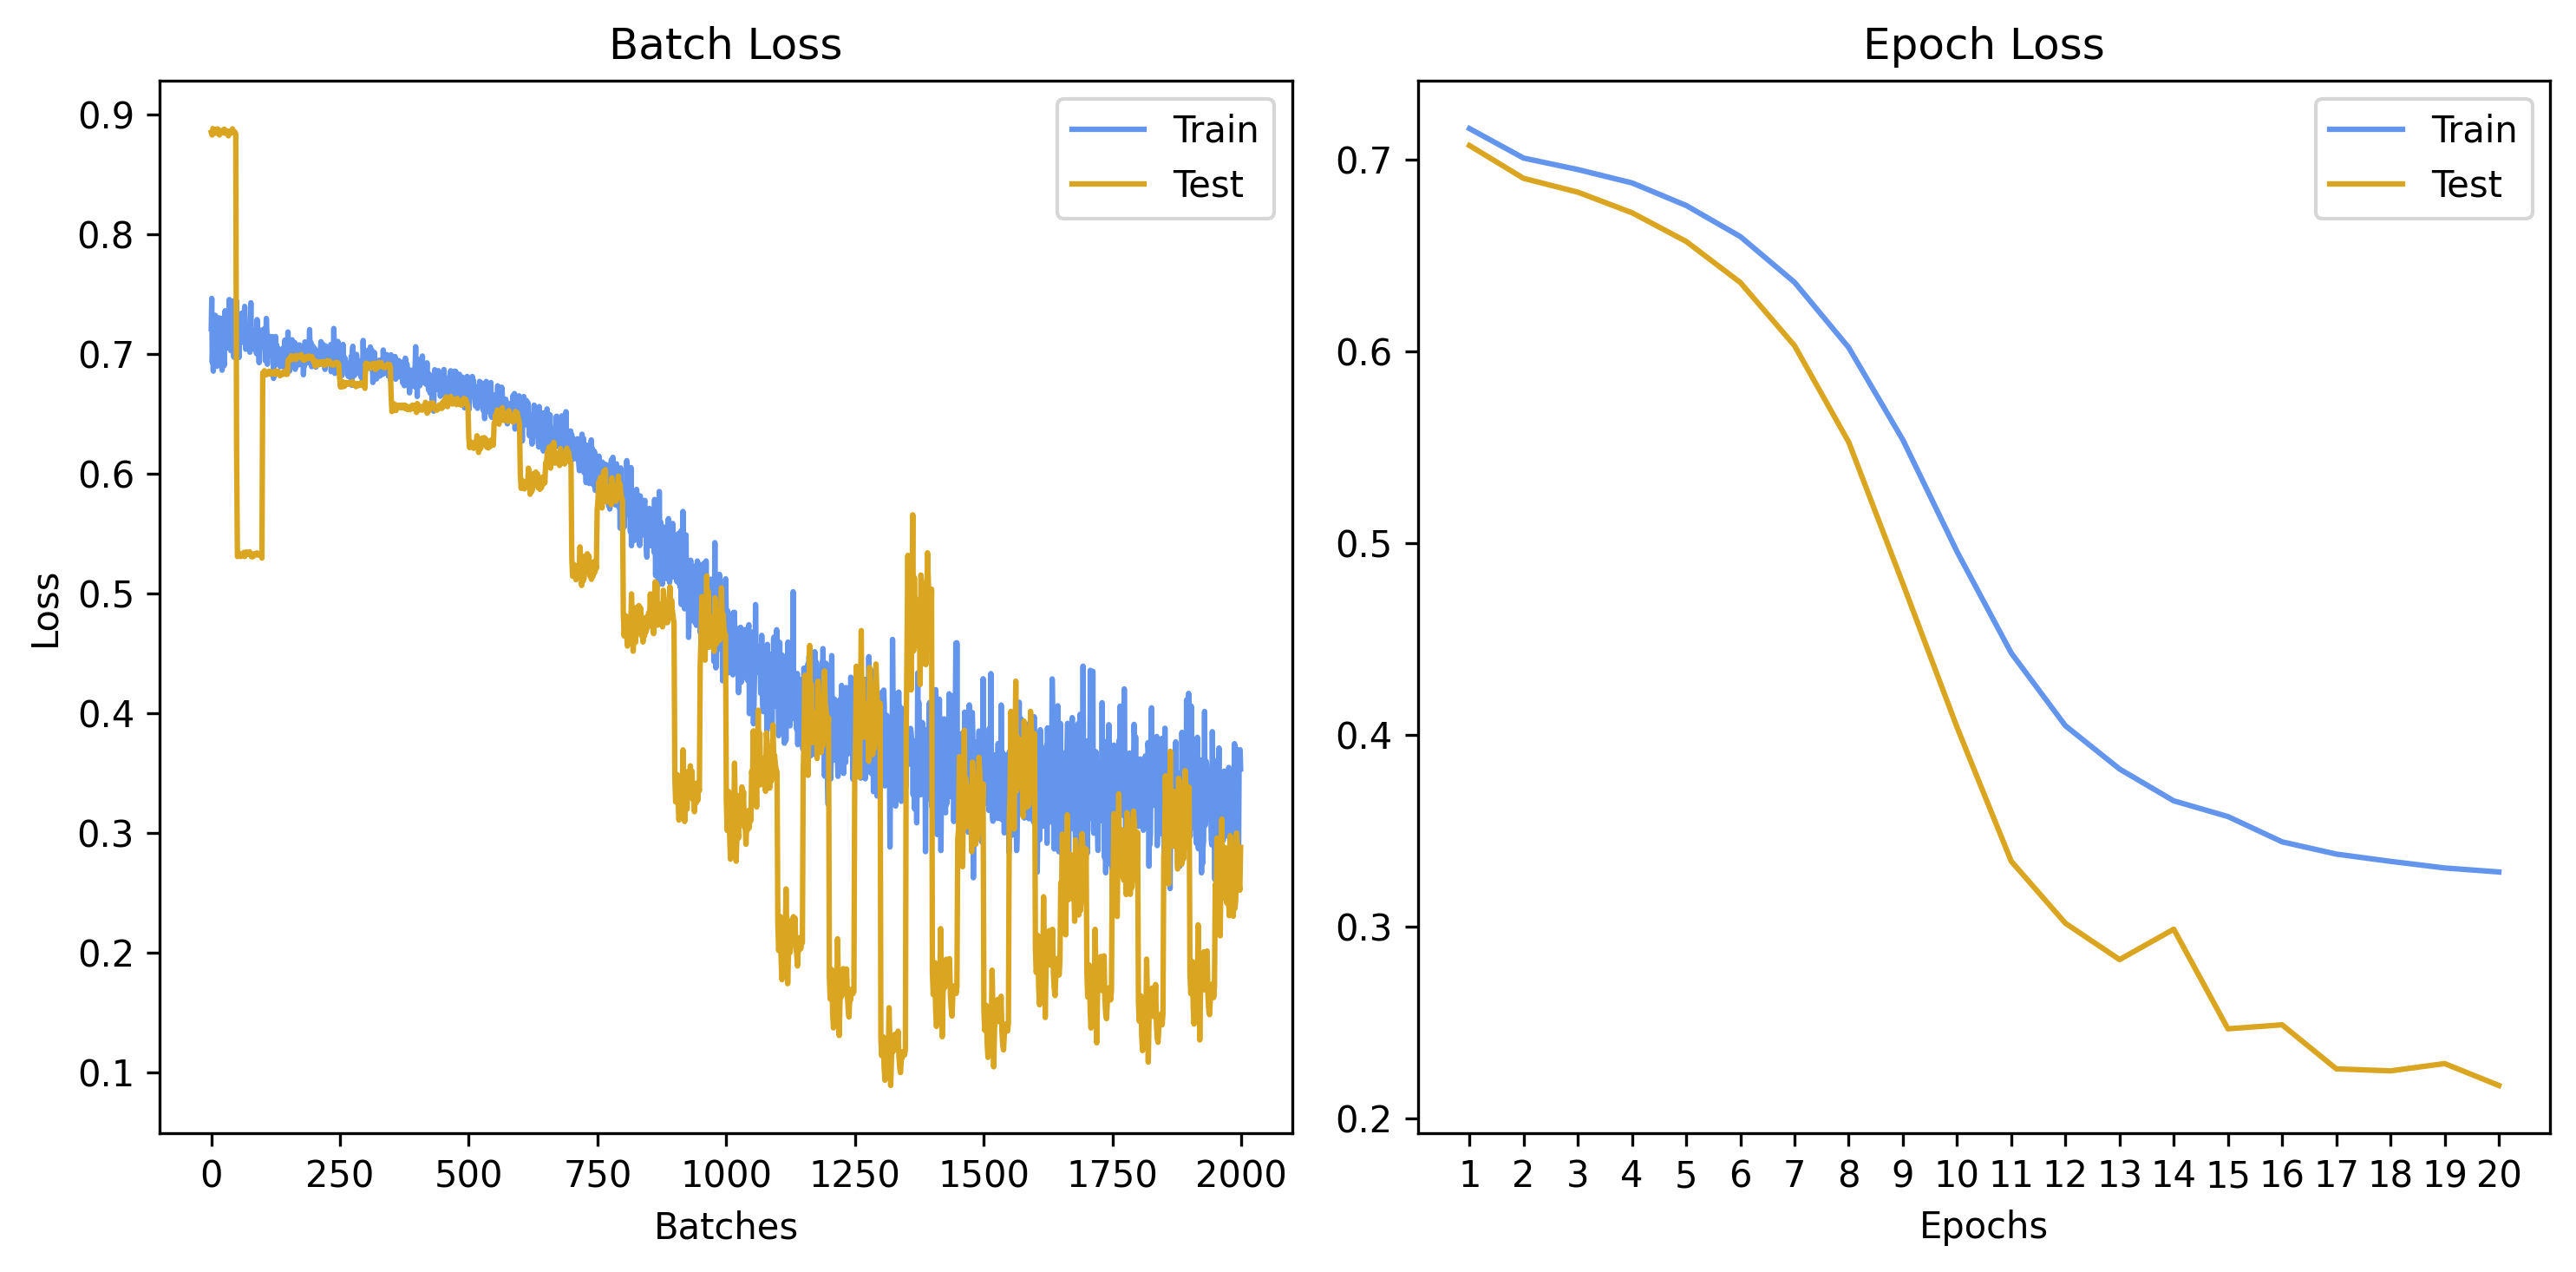
\includegraphics[width=\textwidth]{figures/RoBERTa_learning_curves_1.png}
  \caption{Loss over training}
  \label{fig:roberta-learning-1}
\end{figure}

\begin{figure}
  \centering
  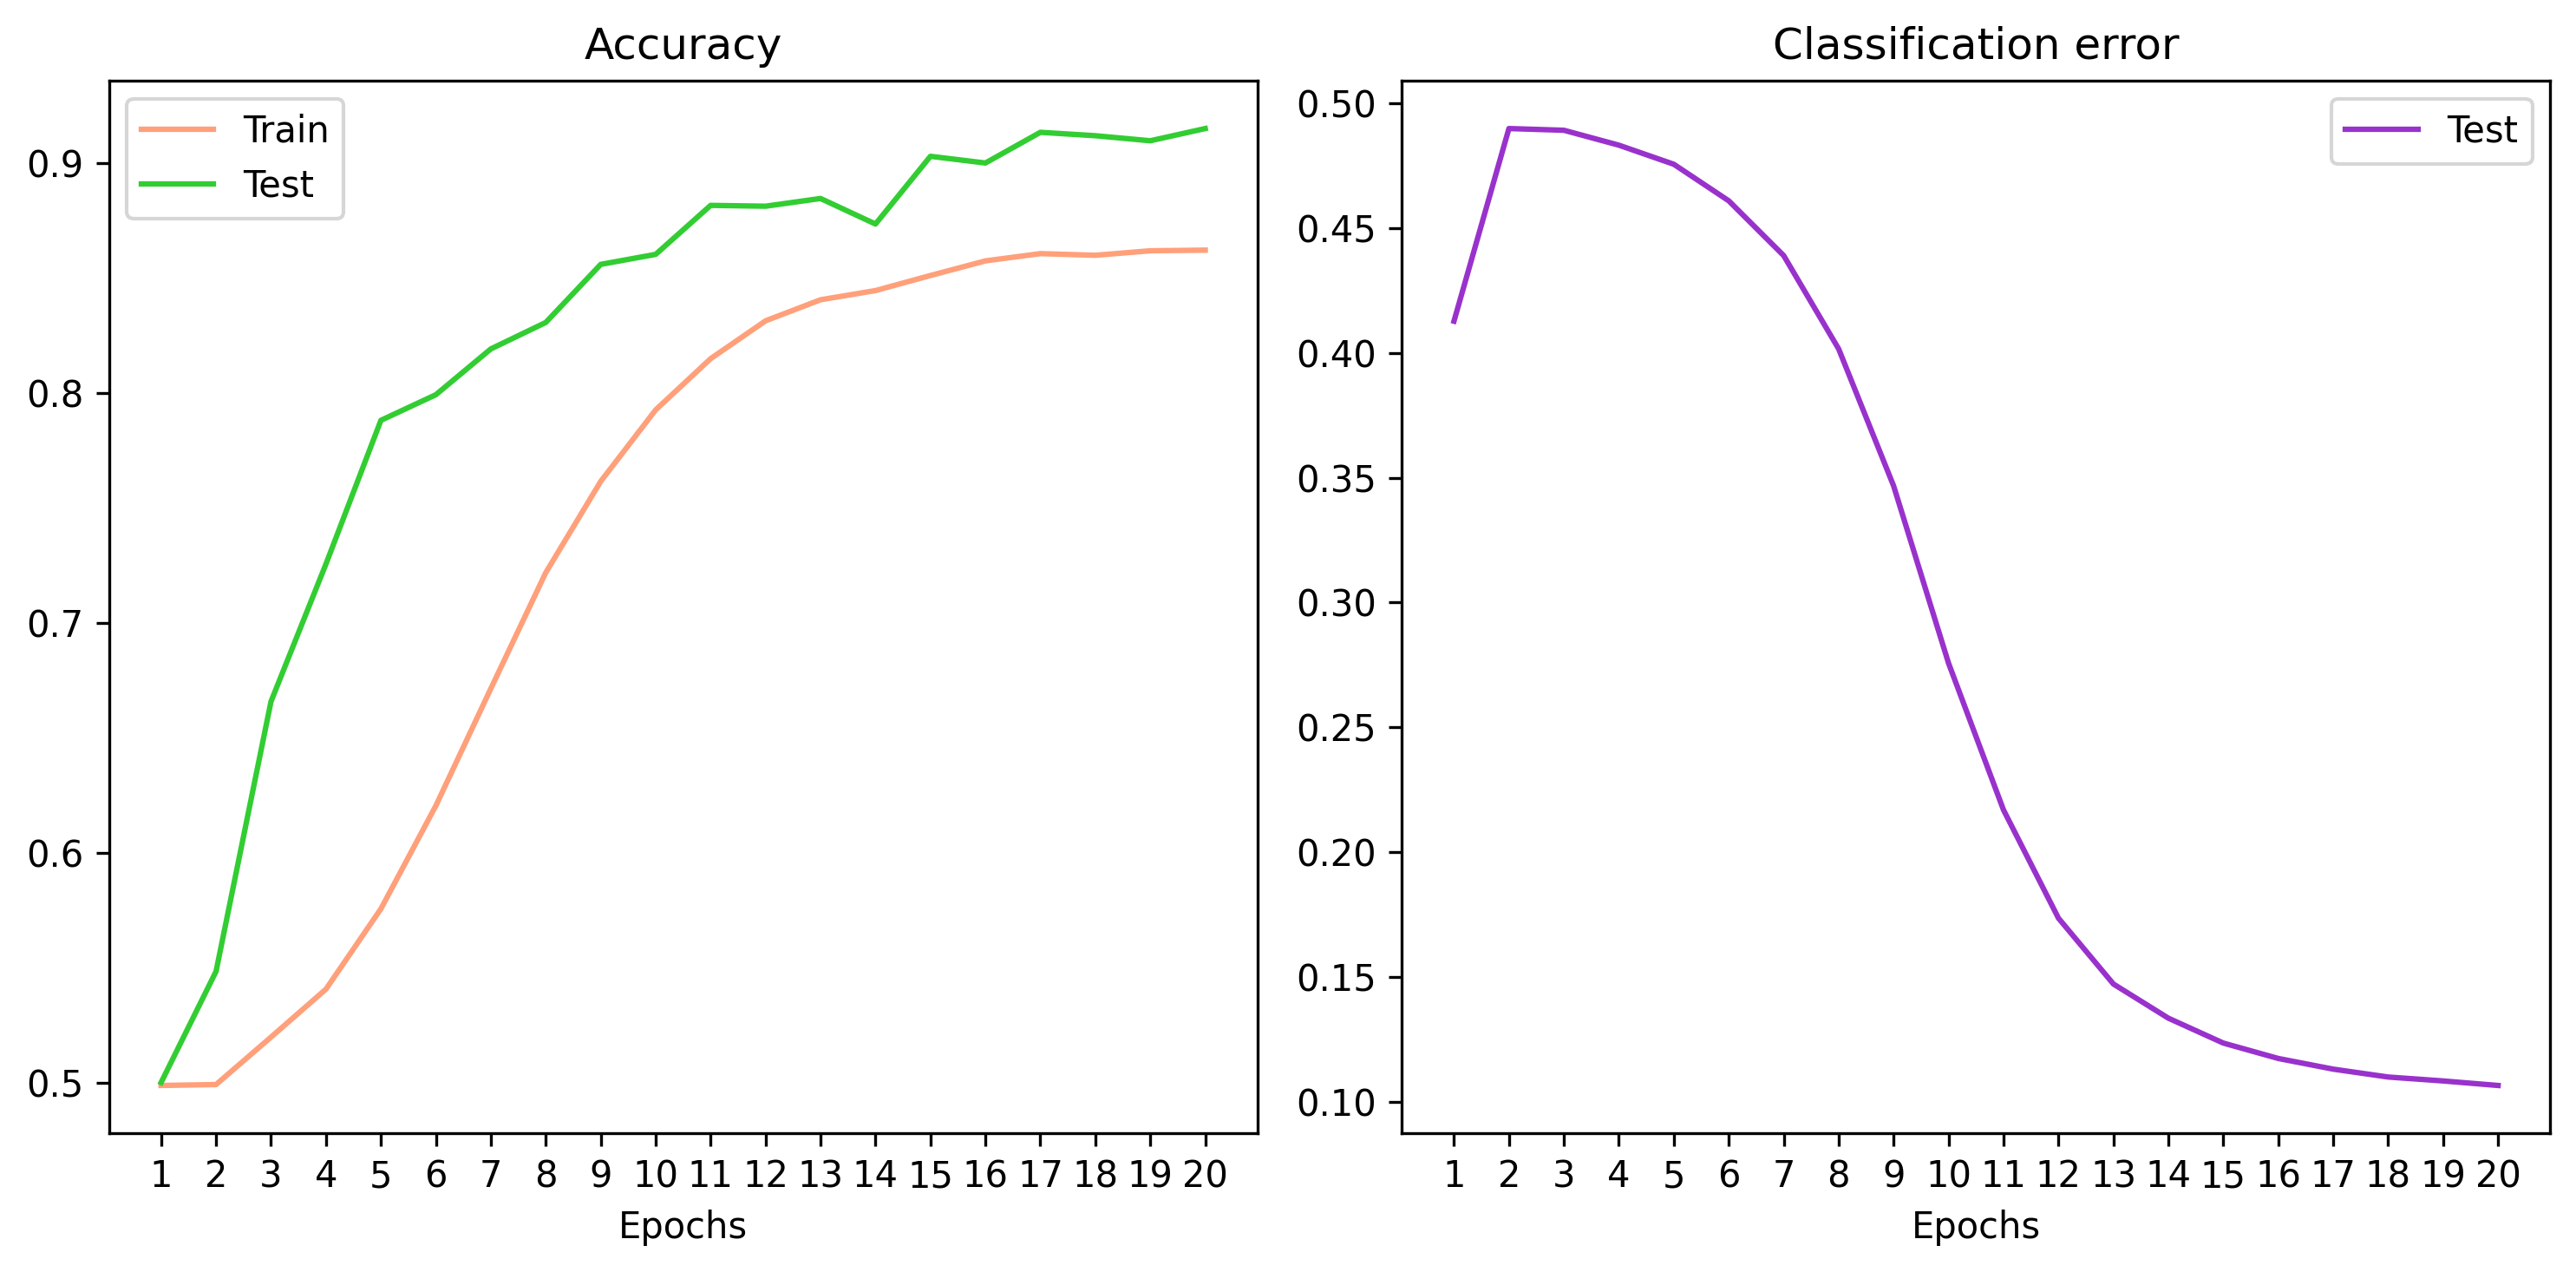
\includegraphics[width=\textwidth]{figures/RoBERTa_learning_curves_2.png}
  \caption{Performance over training}
  \label{fig:roberta-learning-2}
\end{figure}

The effect of training is notable on accuracy, but also on classification error, which reflects the separation between predicted classes, that is, the model confidence in its own predictions (see Figure~\ref{fig:roberta-learning-2}). Classification error is defined as the average difference between the highest possible probability (\( =1 \)) and the highest predicted probability of each datapoint (so the more certain are the label assignments, the closer \( E \) gets to 0):

\[
E = \frac{1}{N} \sum_{i=1}^{N} (1 - P_{\text{max},i})
\]

The overall improvement from fine-tuning is disappointing. While accuracy progresses significantly during training—from 0.5 after the first epoch (equivalent to random guessing, as the dataset is balanced) to 0.9152 after the 20\textsuperscript{th} epoch—it still falls short of the performance achieved by the base model with zero-shot classification, which is already at 0.9158. Moreover, it remains far below the performance of SiEBERT (0.9573) and the SOTA model (0.9668). Several explanations can be envisioned.
\begin{itemize}
    \item The IMDb dataset is too small. Indeed, SiEBERT and the SOTA model are fine-tuned on bigger datasets. But it remains puzzling that even 20 epochs of fine-tuning does not yield better performance than the base model.
    \item My classification head is inadequate, possibly too complex. I tested an alternative model inspired by RoBERTa’s default classification head, consisting of only 2 dense layers with a hidden size of 512. However, the performances of this model were notably worse after 12 epochs (0.8405 accuracy vs. 0.8841 for the original model, and 0.4195 vs. 0.2735 for classification error).
    \item The model did not converge properly. Indeed, 20 epochs seems to be quite a lot for fine-tuning, as typical values range between 3-5 epochs. However, the learning rate was relatively high, and warm-up steps were included, which makes that behavior somewhat perplexing (for reference, the values mentioned in the SOTA article for fine-tuning RoBERTa are 5 epochs with \texttt{lr=1e-6} and \texttt{weight\_decay=0.01} \citep{csanady_llambert_2024}). Maybe the model got stuck in a local minimum.
\end{itemize}

I am unsure what else could have been done. I have reviewed many tutorials on fine-tuning BERT and RoBERTa, but none explicitly addressed its impact on accuracy---especially in comparison to zero-shot classification with optimized prompting. Investigating further was not possible due to the high computational cost. Perhaps fine-tuning RoBERTa \textit{effectively} is harder than it seems 
\footnote{I realized too late that there was a way to significantly speed up training. When the parameters of the base model are frozen, it generates the same embeddings regardless of the training process. So, instead of performing a full forward pass at each epoch, it's possible to feed the input to the base model during preprocessing, store the resulting embeddings, and use them directly for fine-tuning. This approach should reduce computation time to just a few minutes per epoch, as the only remaining task would be to fit a simple neural network on the single token (CLS) for each sequence. Curiously, I found no mention of this trick during my research.}
.

\subsection{Performances}

I have introduced the performance of all models except GPT-3.5 Turbo (see Table~\ref{tab:perfs_by_sentiment}). Its accuracy falls between zero-shot classification with optimized prompting and SiEBERT, highlighting that despite its capabilities and the use of advanced prompting techniques, specialized encoders can still outperform it. It would have been valuable to explore alternative prompt engineering strategies and test other GPT models. However, this was impractical due to the cost and the API's slow speed--—averaging 8 seconds per call, resulting in over 55 hours to process the entire dataset.


\begin{table}
  \caption{Performances of each model}
  \label{tab:perfs_by_sentiment}
  \centering
  \begin{tabular}{lccc}
    \toprule
    \multirow{2}{*}{\centering \textbf{Model}} & \multicolumn{2}{c}{\textbf{Sentiment}} & \multirow{2}{*}{\centering \textbf{Average}} \\
    \cmidrule{2-3}
    & Negative & Positive \\
    \midrule
    RoBERTa fine-tuned & 0.8926 & 0.9378 & 0.9152 \\
    RoBERTa base & 0.8710 & 0.9631 & 0.9171 \\
    GPT & 0.9623 & 0.8978 & 0.9300 \\
    SiEBERT & 0.9520 & 0.9626 & 0.9573 \\
    \bottomrule
  \end{tabular}
\end{table}

\subsubsection{By ratings}

A clear drop in performance is evident for ratings closer to neutral, as expected (see Figure~\ref{fig:accuracy-ratings}). However, the models exhibit notably different behaviors. The accuracy of RoBERTa-base, fine-tuned RoBERTa, and GPT-3.5 Turbo varies with the valence of reviews. RoBERTa-base and fine-tuned RoBERTa perform significantly better on positive reviews than on negative ones, whereas GPT-3.5 Turbo shows the opposite trend, excelling on negative reviews. These models also experience the largest performance declines on their weaker side: -31.9\% for RoBERTa-base, -25.1\% for fine-tuned RoBERTa, and -25.1\% for GPT-3.5 Turbo. SiEBERT, on the other hand, maintains similar performance for both negative and positive reviews, with comparable declines near neutral ratings. This consistency makes it not only the best-performing model but also the most stable across sentiment extremes 
\footnote{This sheds a new light on the effects of fine-tuning. While it improved performance on negative reviews, it reduced it to a larger extent on positive ones. As a result, fine-tuning made the model more consistent, though not better overall.}
\textsuperscript{,}
\footnote{Regarding the GPT model, providing more positive examples than negative one in the prompt could have helped balance its performance.}
.

\begin{figure}
  \centering
  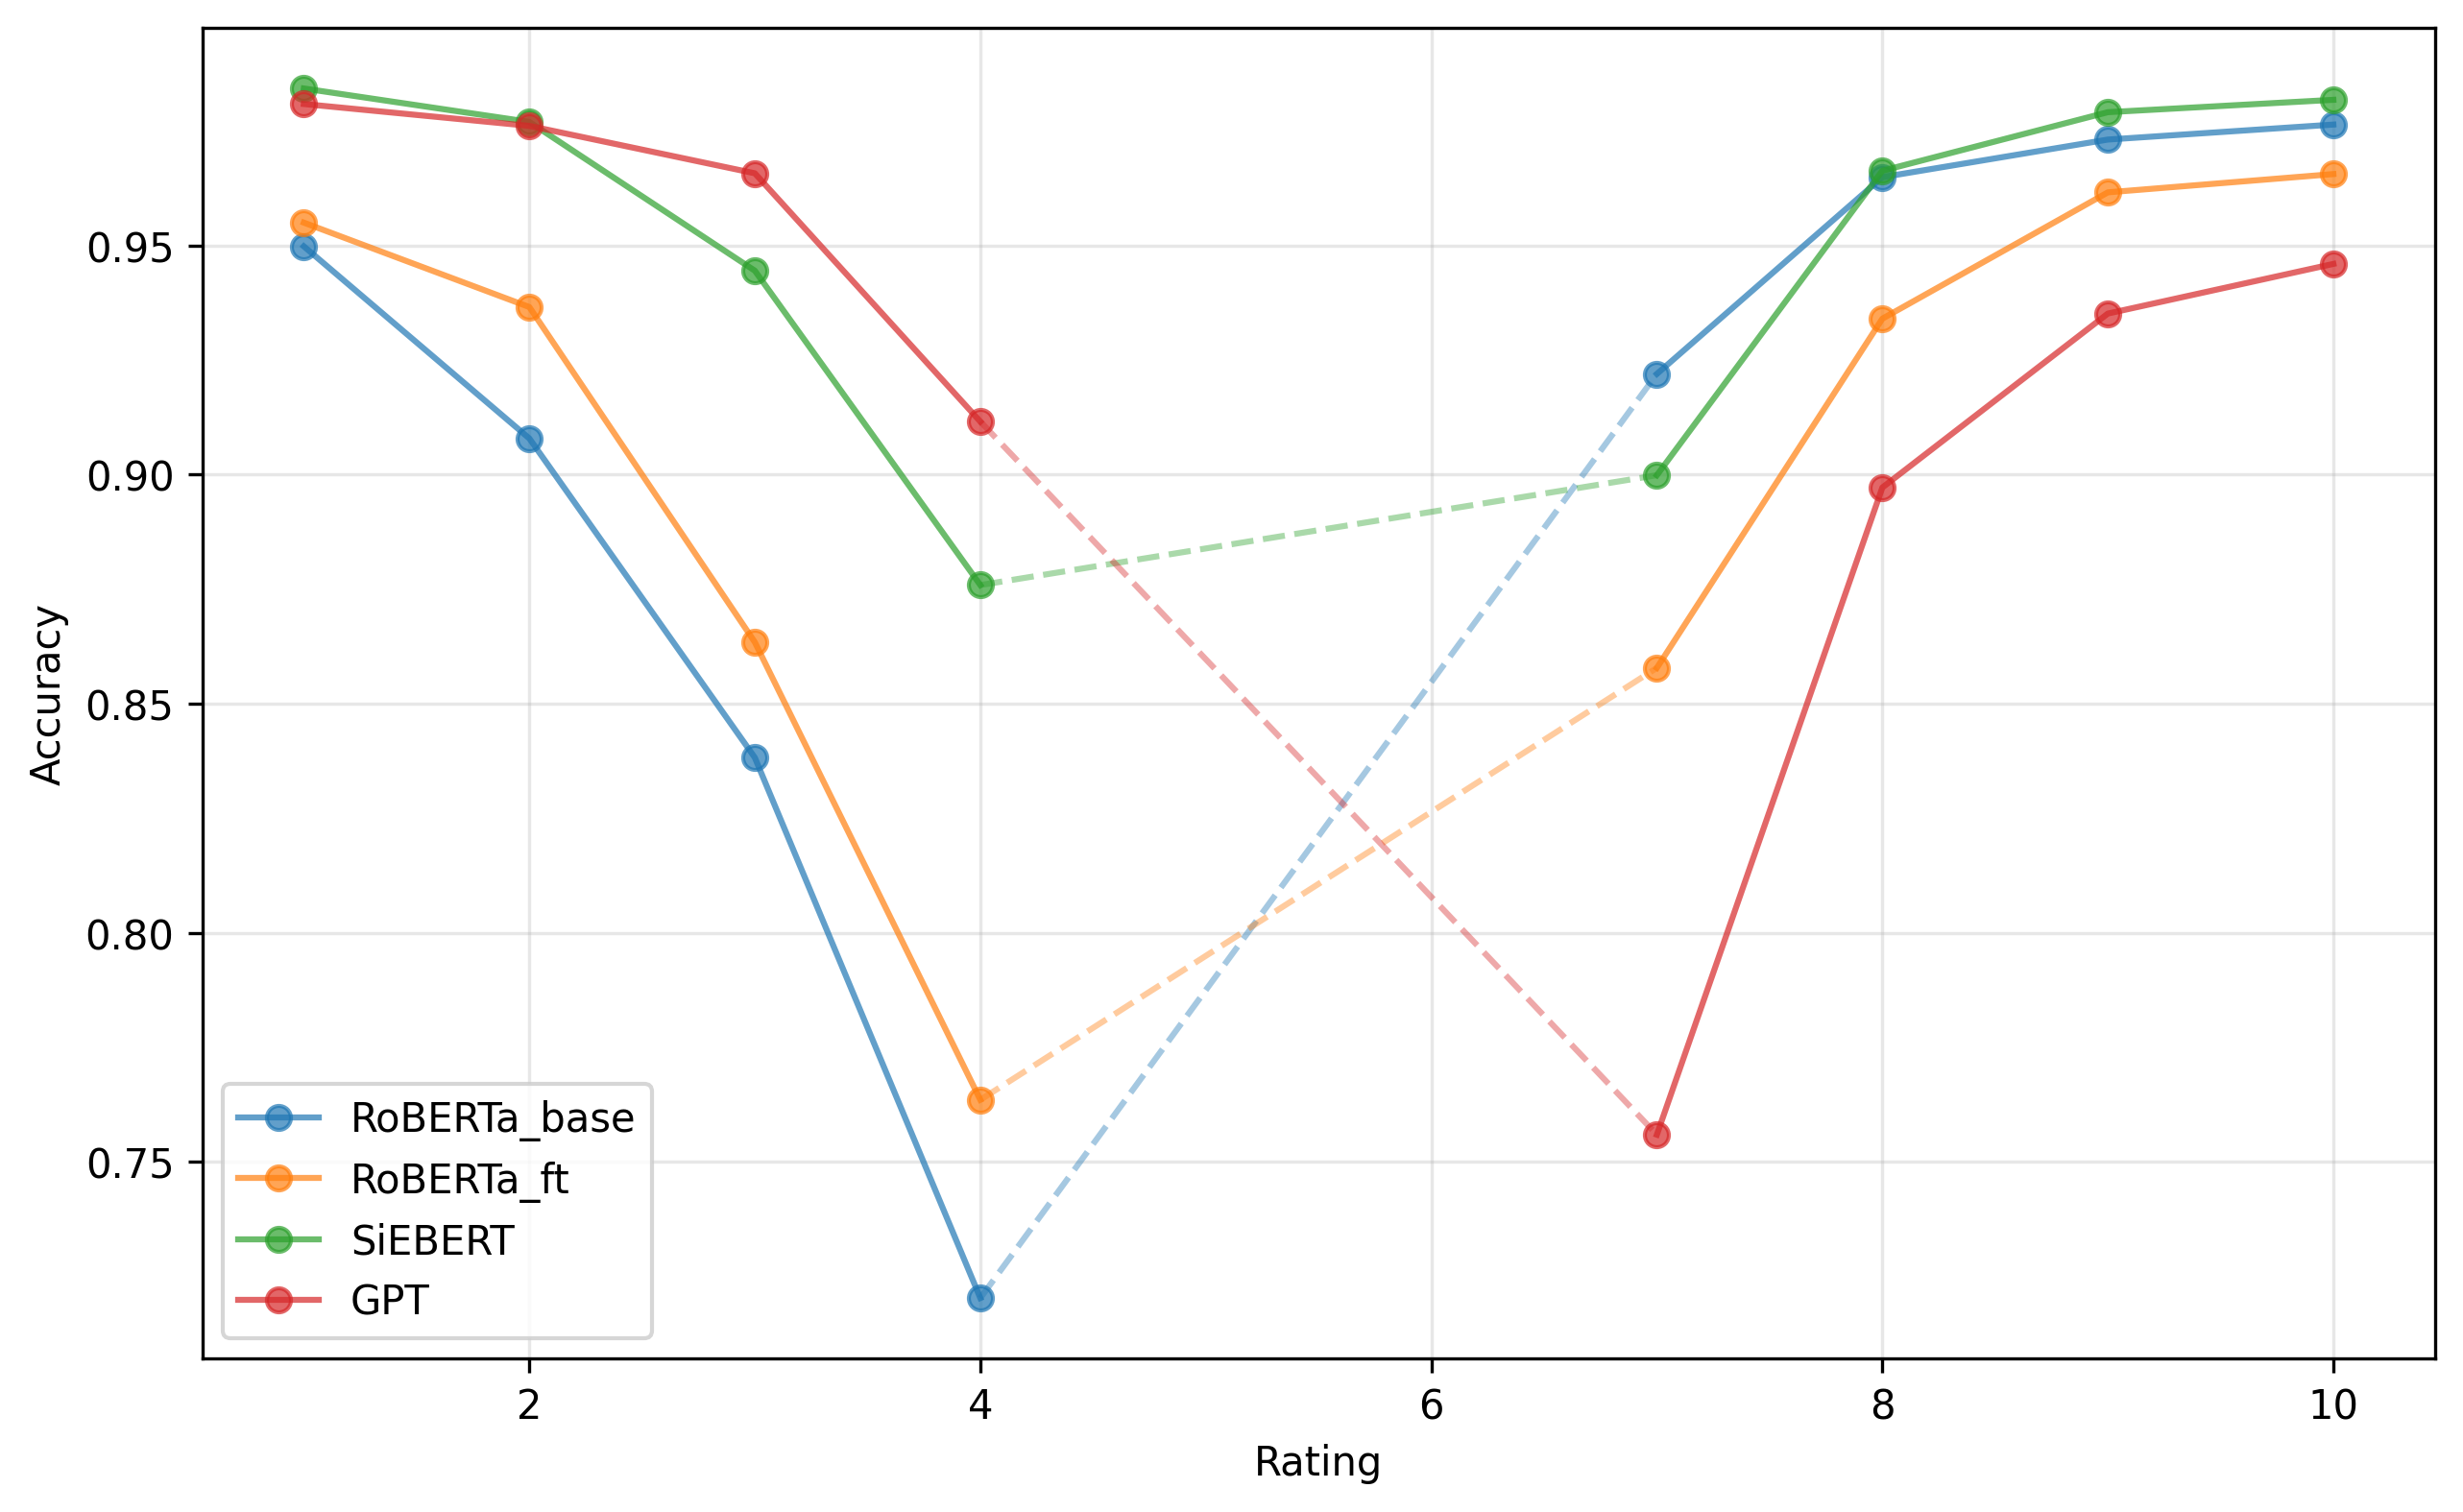
\includegraphics[width=\textwidth]{figures/accuracy_vs_ratings.png}
  \caption{Accuracy by rating}
  \label{fig:accuracy-ratings}
\end{figure}

\subsubsection{By review length}

Similar observations emerge: SiEBERT maintains stable performance, while other models show a clear downward trend, though the effect of review length is much smaller than that of review valence (see Figure~\ref{fig:accuracy-length}). This aligns with the observation that truncation had minimal impact, suggesting that the key information in reviews is not heavily dependent on their length.

\begin{figure}
  \centering
  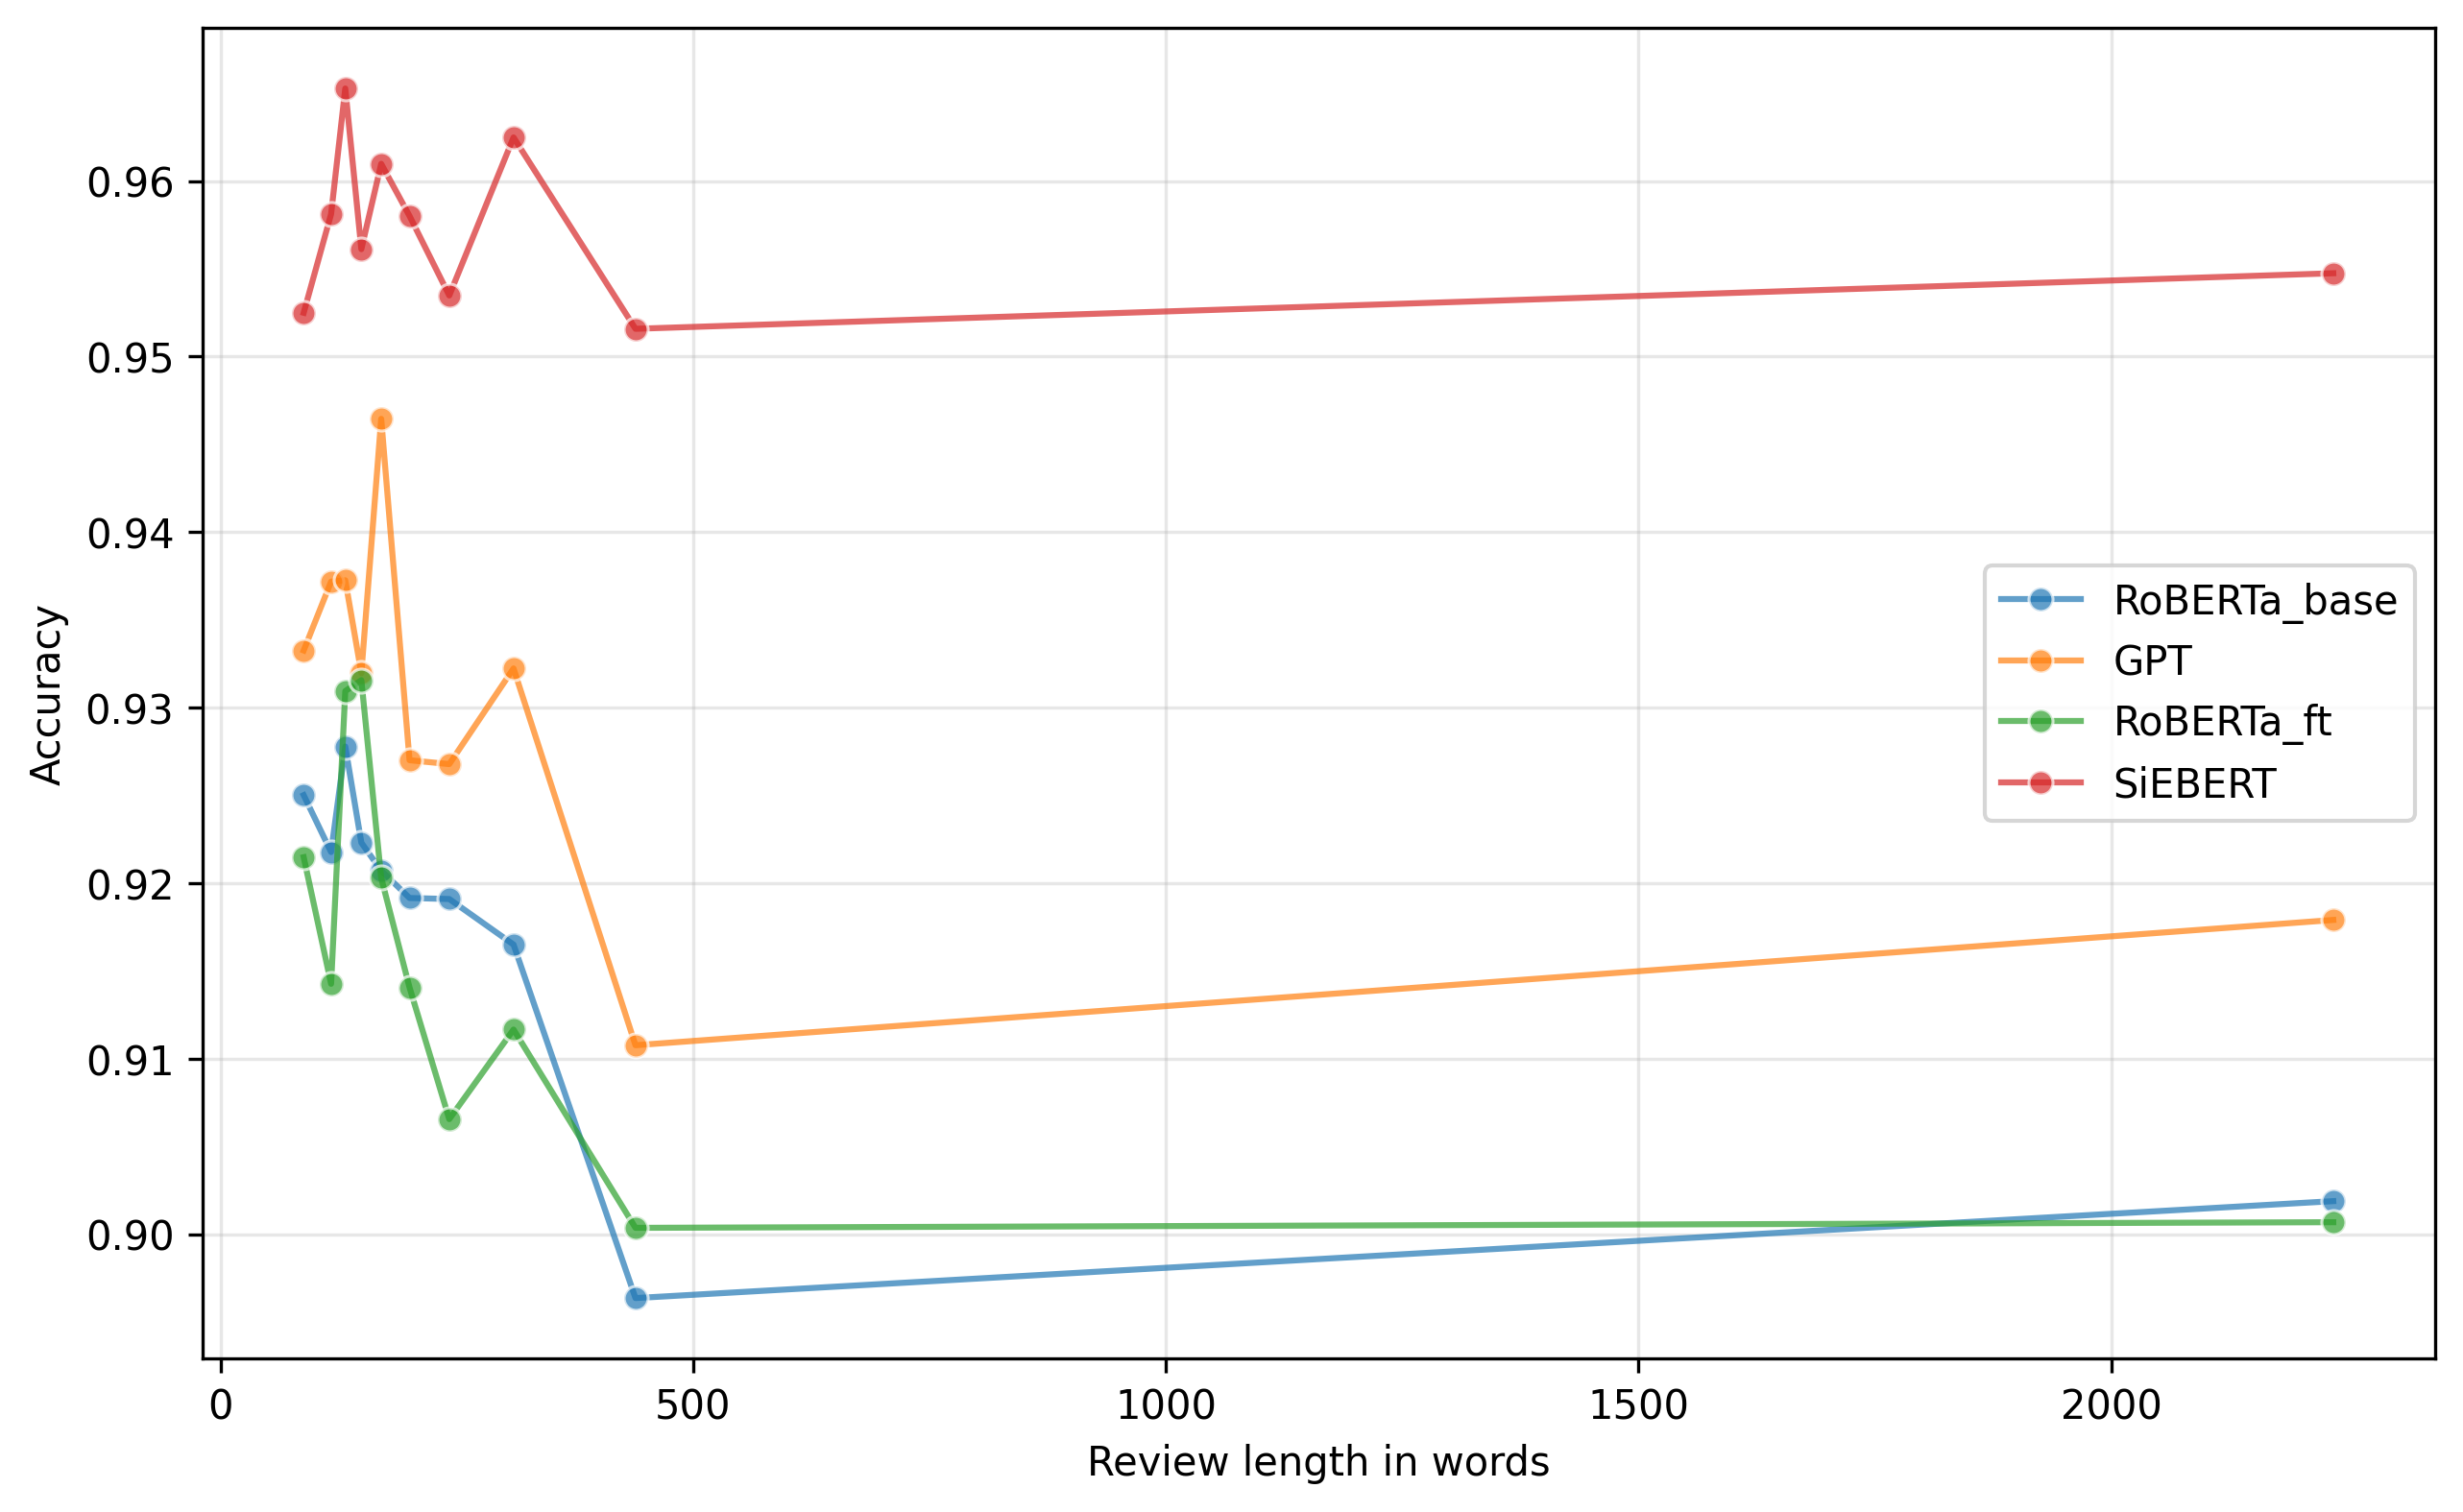
\includegraphics[width=\textwidth]{figures/accuracy_vs_wordcount.png}
  \caption{Accuracy by review length}
  \label{fig:accuracy-length}
\end{figure}

\section{Discussion}

The question addressed in this report was: is the IMDb dataset a limiting factor, responsible for the plateauing of SOTA performance?

The first hypothesis---that noise in the true labels arises because ratings are an imperfect proxy for sentiment---is supported by the fact that accuracy drops significantly for all models when classifying reviews associated with ratings of 4 and 7. One could argue that this phenomenon is perfectly normal: these reviews are harder to classify because they express more nuanced sentiments and are less polarized, making them intrinsically more challenging for models. However, the dataset’s authors somewhat undermine this argument by explicitly excluding reviews deemed too close to neutral, with the explicit aim of focusing on highly polarized reviews. So maybe reviews associated with ratings of 4 and 7 should be excluded as well. This illustrates a fundamental challenge in constructing labeled datasets. Automating the labeling process is tempting, as manual annotation can be as tedious as building a sentiment lexicon. However, automation carries the risk of producing inaccurate or inadequate labels. In such circumstances, an insightful extension would have been to include reviews spanning the full range of ratings and then: (1) examine whether models indeed struggle more with reviews associated with ratings of 5 and 6, and (2) introduce a third category for ternary classification. This category could be defined as \enquote{mixed} instead of \enquote{neutral}, which could prove especially useful for reviews expressing conflicted sentiments (\enquote{I really liked the plot, but the acting was catastrophic…}).

The second hypothesis---that longer reviews are harder to classify---is also confirmed, albeit the corresponding effect is much smaller. The logical extension here would be to shift toward aspect-level sentiment analysis, identifying which aspects of a movie are viewed positively and which are viewed negatively. While significantly more complex, this would be more insightful than simply characterizing the overall tone, and likely represents the future of sentiment analysis for lengthy documents.

\bibliographystyle{unsrtnat}
\bibliography{references}

\end{document}